\newpage
\section{Preventivo a finire} \label{PreventivoFinire}

In questa sezione viene presentato il preventivo a finire. Gli scostamenti rispetto al \hyperref[Preventivo]{preventivo iniziale} sono derivati dal consuntivo dei periodi analizzati precedentemente e dalle modifiche alla pianificazione e ai costi futuri, considerate migliorative per il periodo rimanente. In questa sezione verrà preso in considerazione solo il preventivo per i periodi a carico del committente e si considereranno quelli a carico del gruppo solo per eventuali considerazioni per modifiche alla programmazione futura.

\subsection{Tabella riepilogativa}
\begin{table}[h!]
	\centerline{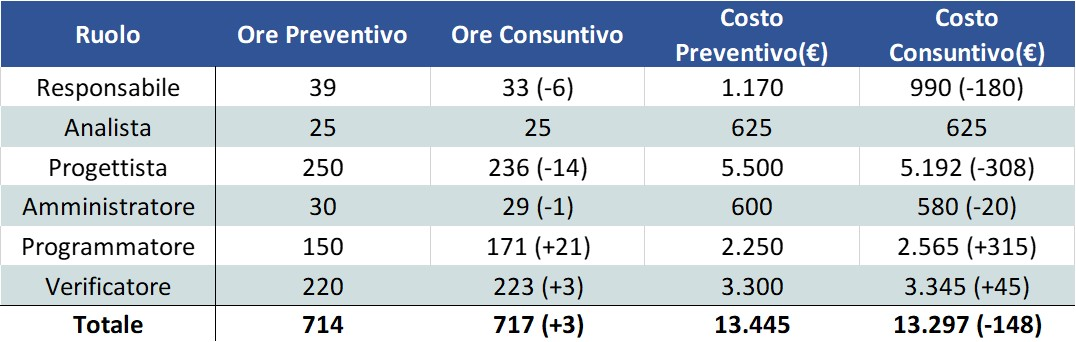
\includegraphics[scale=0.60]{img/Preventivo/Consuntivo/PreventivoFinire.jpg}}
	\caption{Preventivo a finire}
\end{table}

\subsection{Conclusioni}
Rispetto al preventivo iniziale, sono state effettuate alcune modifiche in seguito al consuntivo riguardante il periodo di Prototipazione. Oltre agli scostamenti rilevati nel periodo appena citato, sono state assegnate ulteriori 10 ore ai \progrs{} a discapito dei \progs{} in previsione dei periodi a venire. Questo si traduce in un risparmio per il committente pari a \EUR{210} e quindi un costo totale rendicontato del preventivo a finire pari a \EUR{13.235}.